\documentclass[]{article}

\usepackage{fullpage} % Package to use full page
\usepackage{parskip} % Package to tweak paragraph skipping
\usepackage{tikz} % Package for drawing
\usepackage{amsmath}
\usepackage{hyperref}

\title{Arduino Capacitance Meter}
\author{Dr. Matthew Riehl}
\date {\today}

\begin{document}
\newcommand{\ds}{\displaystyle}
\maketitle

\section{Introduction}

This week, you will build a capacitance meter  to measure the capacitance of unknown capacitors.  In addition, you will study the equivalent capacitance of capacitors in series and in parallel.  The lab can be open-ended and you are encouraged to find ways to improve the circuit and code to make a more versatile instrument.

\section{Materials}
The materials below were assembled earlier to display a brief message from the Arduino on the LCD.  Check to ensure that the board is still assembled and that the display still works.  If it does not, your first job is to fix it.
\begin{itemize}
	\item PC with Arduino IDE installed (provided, but you may use your own).
	\item Arduino Uno board and power cable
	\item Half-size breadboard
	\item LCD display module
	\item 220 $\Omega$ resistor ($\Omega$ is Ohm)
	\item 10 k$\Omega$ potentiometer
	\item Jumper wires
\end{itemize}
The materials here are the new parts needed for completion of this weeks project.
\begin{itemize}
	\item Jumper wires
	\item Resistors (various sizes)
	\item Capacitors, also various sizes
\end{itemize}

\section{Background}
A parallel plate capacitor was introduced earlier to describe a device that generated a uniform electric field.  A simple schematic of such a capacitor is shown in Figure \ref{capacitor}.  While a uniform electric field is a useful thing, this is not why capacitors are found in many electronic circuits.  Rather, capacitors are useful because they can be charged, store electrical energy, and discharged faster than a chemical battery.  For example, the flash on a camera requires a large electric current in a  short pulse.  A battery is unable to produce enough current to create a bright flash, so the battery is used to charge a capacitor which  then  discharges the stored energy  quickly (\dots \emph{in a flash!}).  Another common use is in electric motors.  It takes more work to initially start the motor than it takes to maintain the rpm once it is moving.  Capacitors can provide an initial burst of energy to accelerate the motor.




\begin{figure}[h]
\begin{center}
	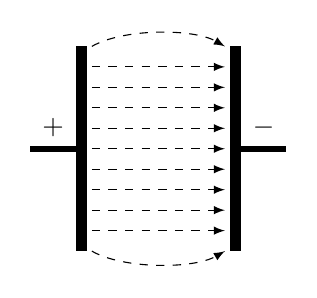
\begin{tikzpicture}[scale=0.65, >=latex]
		\draw[line width=2] (1.0,0) -- (0,0) node[above right] {$+$};
		\draw[line width=4] (1.0, 2,0) -- (1.0, -2.0);
		\draw[dashed,->] (1.2,2.0) to[looseness=.7,bend left=30] (3.8,2.0);
		\foreach \y in {-1.6,-1.2,-0.8,...,1.6} 
			\draw[dashed, ->] (1.2, \y) -- (3.8, \y);
		\draw[dashed,->] (1.2,-2.0) to[looseness=.7,bend right=30] (3.8,-2.0);
		\draw[line width=2] (4.,0) -- (5.0,0) node[above left] {$-$};
		\draw[line width=4] (4.0, 2,0) -- (4.0, -2.0);
	\end{tikzpicture}
	\caption{Parallel Plate Capacitor}
	\label{capacitor}	
\end{center}
\end{figure}

Unlike a battery, which is charged and discharged according to the rate of a chemical reaction, a capacitor can be charged or discharged very quickly -- especially useful when powering a camera flash, an AED, or a taser.  The factor that limits how quickly a capacitor charges or discharges, besides its size, is the resistance in the circuit, which limits the current and how quickly charge can build up on the capacitor.  If a capacitor is initially uncharged, the charge builds rapidly at first, but as the voltage on the capacitor approaches the potential of the source, the rate of charging slows down.  A plot of charge vs. time is shown in Figure \ref{charge}.  

\begin{figure}[h]
	\begin{center}
		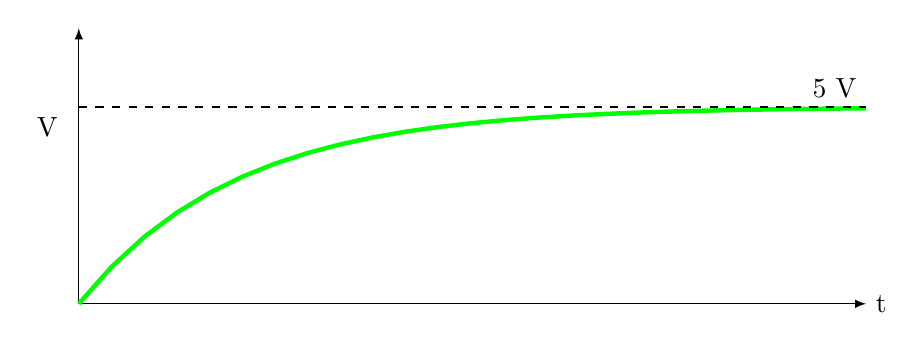
\begin{tikzpicture}[xscale=20,yscale=5,>=latex]
		\draw [<->] (0,0.7) -- (0,0) -- (0.5,0) node[right] {t};
		\node at (-0.02,.45) {V};
		\draw[green, ultra thick, domain=0:.5] plot (\x, { .5 * (1 - exp(-1*\x / 0.10))});
		\draw [dashed] (0,.5) -- (.5,.5) node[above left] {5 V};
		\end{tikzpicture}
		\caption{Capacitor charging}
		\label{charge}
	\end{center}
\end{figure}

Similarly, the rate at which the capacitor discharges depends on the resistance in the circuit.  In Figure \ref{discharge} below, three discharge curves are shown, the red illustrates the discharge in a circuit with  little resistance,  and the blue a circuit with a  large resistance.

\begin{figure}[h]
	\begin{center}
		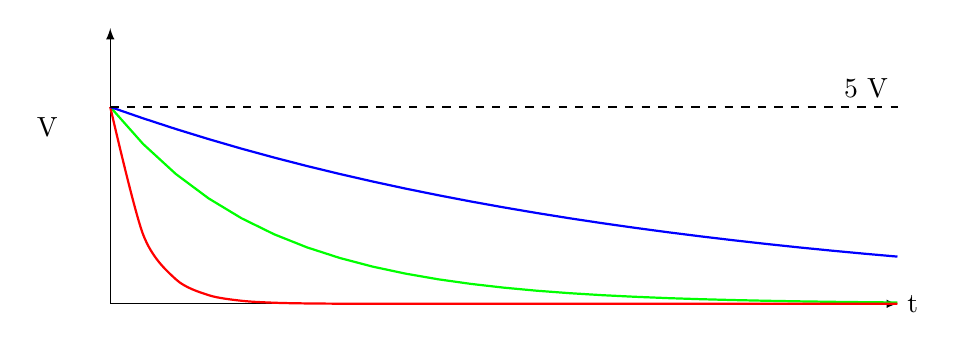
\begin{tikzpicture}[xscale=20,yscale=5,>=latex]
		\draw [<->] (0,.7) -- (0,0) -- (0.5,0) node[right] {t};
		\node at (-0.04,.45) {V};
		\draw[green, thick, domain=0:.5] plot (\x, { .5 * ( exp(-1*\x / 0.10))});
		\draw[smooth, red, thick, domain=0:.5] plot (\x, { .5 * ( exp(-1*\x / 0.02))});
		\draw[blue, thick, domain=0:.5] plot (\x, { .5 * ( exp(-1*\x / 0.35))});
		\draw [dashed] (0,.5) -- (.5,.5) node[above left] {5 V};
		\end{tikzpicture}
		\caption{Capacitors discharging}
		\label{discharge}
	\end{center}
\end{figure}

These charge and discharge curves are modeled by the equations:
 \begin{equation*}
 q=q_0\left[1-e^{-t/(RC)}\right] \qquad\qquad \text{Charging the Capacitor}
 \end{equation*}
and 
\begin{equation*}
q=q_0e^{-t/(RC)}  \qquad\qquad \text{Discharging the Capacitor}
\end{equation*}

where $q_0$ is the maximum voltage, $R$ is the resistance in the circuit and $C$ is the capacitance of the capacitor in Farads.  The product $RC$ is called the time constant, which is $\tau$:  $\tau=RC$.  This equation provides a way to measure the capacitance of any capacitor.  If a fully discharged capacitor is charged, when  $t=\tau$, $\ds q = q_0 \times [1-e^{-1}]$, or $q=q_0 \times 0.632$.  Note that the time constant depends on the capacitance of the capacitor \emph{and} the resistance in the circuit.  

Figure \ref{cap} is a simple schematic of the circuit you will build this week.  The Arduino provides the voltage to charge the capacitor and controls the three switches.  In addition, it measures the charge on the capacitor (the voltage) as a function of time, using its built in timer.  When the program starts, the charging switch is in the `closed' position, allowing current to flow to the capacitor while the Arduino monitors the voltage as a function of time.  The $10k \Omega$ resistor limits the current and slows the charging, otherwise the capacitor may charge too quickly to measure. (You will choose the resistor in the circuit and modify the Arduino program to reflect the resistance used.) When the voltage reads 3.16 volts ($3.16 V = 5 V \times 0.632$), the Arduino calculates the capacitance from $t=\tau=RC$: 
\begin{equation*}
C=\frac{t}{R}=\frac{t}{10000} 
\end{equation*}

To discharge the capacitor, the Charging switch is opened and the `Discharge through LED' switch is closed.  Only one discharge circuit is needed, but the second is helpful since we are inserting an LED into the  discharge circuit.  The initial discharge directs the current through the LED, which will glow briefly.  When the voltage drops below a minimum voltage for the LED, the current essentially stops, and the capacitor discharges only very slowly.  The final discharge switch is then closed to allow the capacitor to finish discharging quickly.  The $1k \Omega$ resistor in this part of the circuit also limits the current and  allows the LED to remain lit for a longer period of time.  You can change this resistor to see how it affects the LED brightness.



\begin{figure}[h]
	\centering
	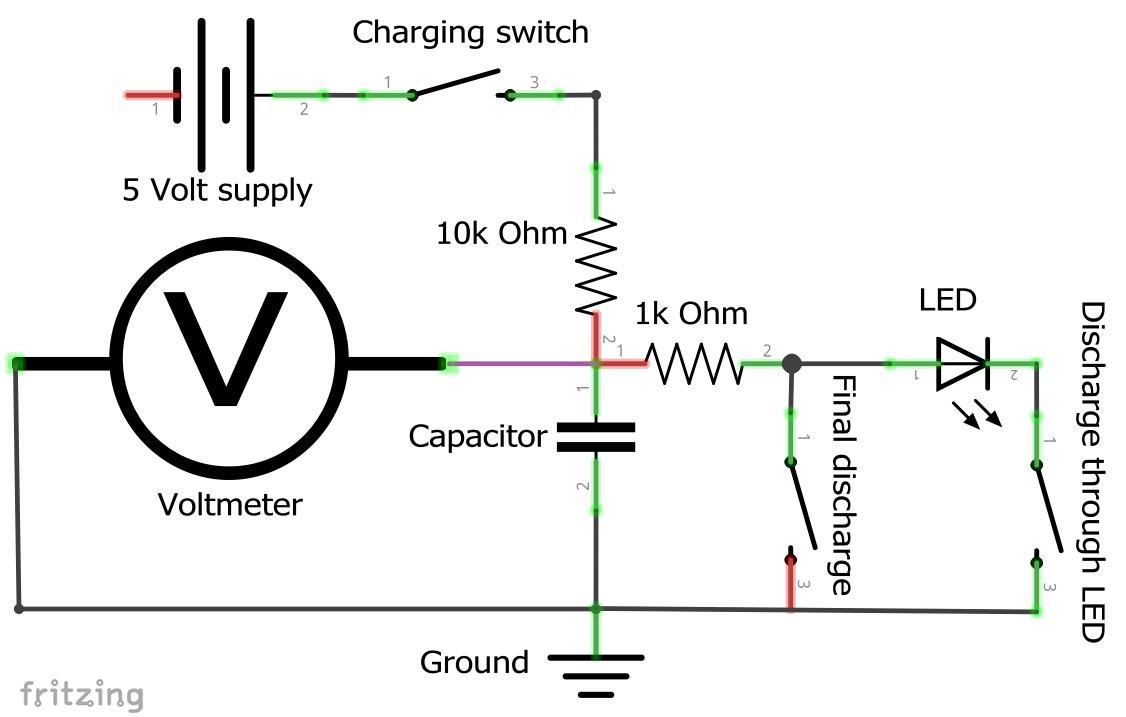
\includegraphics[width=12cm]{pics/Schematic.png}
	\caption{Capacitance Schematic}
	\label{cap}
\end{figure}


\section{Arduino Pinout}

The LCD display you built earlier will not be changed.  The circuit may be easier to work with if you use a second small breadboard for the new circuit, but it is not necessary (Figure \ref{pinout}).  

First, attach the wire that will provide 5.0 V to the capacitor.  Rather than drawing this from the 5V Power pin we have been using, we will use one of the digital pins so we can turn it on and off.  It doesn't matter which one, but the code specifies pin \#\,4 (if you use a different pin, you must also change the given code).  The ground does not need to be turned on and off, so we connect the ground end of the capacitor to the ground we have been using.  

When you insert the capacitor, note that one pin is shorter than the other and may be marked with a \((-)\) sign.  Many capacitors are electrolytic capacitors and cannot be inserted backwards.  The \((-)\) pin must be connected to the ground and the other (longer) pin is connected to the 5\,V power supply.  If it is inserted backwards, the capacitor may be damaged or ruined.  % They can explode, too\dots

You will notice that the LED also has one short pin.  The LED is a diode: a semiconductor device that allows current to flow only in one direction.  Diodes must be inserted so that the current flows from high potential source through the long pin and out the short pin; like the capacitor, the short pin goes to ground.  If this is inserted backwards, the LED won't light, but it also won't be damaged unless the voltage is quite large.  

Since the discharging of the capacitor must be controlled, the discharge wires are connected to the Arduino digital pins.  In this sketch, we are using pin \#\,6 for the discharge through the LED and pin \#\,5 for the final discharge.



	\begin{figure}[h]
		\centering
		\includegraphics[width=16cm]{pics/breadboard.png}
		\caption{Pin-out Diagrams for the Ohmmeter}
		\label{pinout}
	\end{figure}


The resistors are suggested values.  As you experiment with the capacitance meter, you will be able to replace these resistors with others and see how the results are affected.  If the $10\,k \Omega$ resistor is replaced, you will have to update the code and reload it to the Arduino.  The resistor in the discharge circuit has no effect on the operation of the meter and can be changed at any time.  You will note that this resistor affects how long the LED remains lit during discharge and how bright it is.

\section{Code for the Arduino}

The code for this  lab is reproduced below, but is also available in a separate .ino file.  Note that the value of the  resistor is set to $10,000\ \Omega$  (\# define resistorValue).  If your time constant is too long or too short you will need to replace the resistor with a different one, and this line of code will also have to be changed.  You must upload the new code to the Arduino before it takes effect.

Remember that anything after // is a comment.  It gets messy, but read them.  If you have programming experience, you may feel that this is some ugly code -- feel free to improve it!

\begin{verbatim}
/*
This code is included with the files for Arduino Labs Capacitance Meter by 
Matthew Riehl and is in the public domain.  I have only modified the
code to better support the laboratory exercise.  Several Capacitance Meters
are described online.  The original inspiration for this priject is from
https://www.arduino.cc/en/Tutorial/Foundations/CapacitanceMeter,  
https://www.circuitbasics.com/how-to-make-an-arduino-capacitance-meter/, and
https://electronoobs.com/eng_arduino_tut10_1.php.

Note that the pin assignments for the LCD are NOT the same as found on many  
Arduino pages.  They have been moved around to make the wiring more  
intuitive and easier to troubleshoot.

The LCD circuit:
* LCD RS pin to digital pin 7
* LCD Enable pin to digital pin 8
* LCD D4 pin to digital pin 9
* LCD D5 pin to digital pin 10
* LCD D6 pin to digital pin 11
* LCD D7 pin to digital pin 12
* LCD Backlight (pin 15 on LCD) to pin 13 on Arduino (might 
need to add a 220 ohm series resistor)
* LCD R/W pin to ground
* LCD VSS pin to ground
* LCD VCC pin to 5V
* 10K potentiostat:
- ends to +5V and ground
- wiper to LCD VO pin (pin 3)

Additional circuit elements for the Capacitance Meter:
* Arduino pin 4 charges the capacitor
* Arduino pin 5 is ground as the final discharge pin
* Arduino pin 6 is ground for the initial discharge pin
* Arduino pin A0 monitors the voltage across the capacitor
*/

// include the library code:
#include <LiquidCrystal.h>

// initialize the library by associating any needed LCD interface pin
// with the arduino pin number it is connected to
const int rs = 7, en = 8, d4 = 9, d5 = 10, d6 = 11, d7 = 12;
LiquidCrystal lcd(rs, en, d4, d5, d6, d7);

//this section assigns meaningful names to the pins on the Arduino that will be used.  
//It also defines the variable "resistorValue" and assigns it a value of 10000 ohms.

#define analogPin      0          // pin A0
#define chargePin      4         
#define dischargePin   6        
#define dischargePin2  5
#define resistorValue  10000     // Can be changed for different capacitors
#define backlightPin 13         // This allows the user to turn the back light on and off.


//more variables are defined.  
unsigned long startTime;        // unsigned long is an integer that can be larger
unsigned long elapsedTime;      // than a typical int.  If int is used, you might
// end up with a negative number for the capacitance.
float microFarads;              
float nanoFarads;
float voltage=0;

//the actual program begins here.  The charge pin is set as a current source with a
//potential of 0V
void setup()
{
	pinMode(backlightPin, OUTPUT);
	digitalWrite(backlightPin, HIGH);
	pinMode(chargePin, INPUT);     
	pinMode(dischargePin2, OUTPUT);       // To ensure the capacitor is fully discharged 
	digitalWrite(dischargePin2, LOW);     // dischargePin2 is set to ground
	lcd.begin(16, 2); 
	lcd.setCursor(0,0);
	lcd.print("Capacitance");
	lcd.setCursor(0,1);
	lcd.print("Meter!!!");
	delay(3000);
	lcd.clear();
	lcd.setCursor(0,0);                
	lcd.print("R1 Resistance");
	lcd.setCursor(0,1);
	lcd.print(resistorValue);
	lcd.print(" Ohms"); 
	delay(5000);
	while(analogRead(analogPin) > 0) {
	}
	lcd.clear();
	pinMode(dischargePin2, INPUT);
	pinMode(dischargePin, INPUT); 
}

//This loop runs forever
void loop(){
	lcd.clear();
	delay(500);
	lcd.print("Charging....");
	pinMode(chargePin, OUTPUT);           //make sure that the chargePin is a current source
	digitalWrite(chargePin, HIGH);        //sets it to a potential of 5V rather than 0V
	startTime = millis();                 //Look at the clock and record the start time
	while(analogRead(analogPin) < 648){   //Monitor the digital voltage until it equals 648
		voltage = ((analogRead(analogPin))*5.000/1024); //While it's monitoring the voltage, 
		lcd.setCursor(0,1);                             //dispay it on the LCD
		lcd.print("V  = ");
		lcd.print(voltage);        
	}
	
	elapsedTime= millis() - startTime;           //when digital voltage reads 648, calculate 
	microFarads = ((float)elapsedTime / resistorValue) * 1000;   // capacitance
	lcd.clear();
	lcd.print(elapsedTime);                         //first, display the time constant, RC
	lcd.print(" mS");
	delay(2000);  
	lcd.clear();
	//delay(1100);
	
	if (microFarads > 1){                               //calculate and display microFarads
		lcd.print(microFarads);       
		lcd.print(" uF");   
		delay(2000); 
		while(analogRead(analogPin) < 1000) {
			voltage = ((analogRead(analogPin))*5.000/1024);         
			lcd.setCursor(0,1);
			lcd.print("V  = ");
			lcd.print(voltage);  
		}   
	}
	
	else{
		nanoFarads = microFarads * 1000.0;                //or calculate and display nonoFarads
		lcd.print(nanoFarads);         
		lcd.print(" nF");          
		delay(2000); 
		while(analogRead(analogPin) < 1000) {
			voltage = ((analogRead(analogPin))*5.000/1024);         
			lcd.setCursor(0,1);
			lcd.print("V  = ");
			lcd.print(voltage);
		}
	}
	
	//This controls the discharging.  
	lcd.clear(); 
	lcd.print("Discharging.....");
	pinMode(chargePin, INPUT);        //First, the charging pin must be turned off by making 
	pinMode(dischargePin, OUTPUT);    //it an INPUT pin and the first discharge pin is turned 
	digitalWrite(dischargePin, LOW);  //into OUTPUT and set to 0V so the charge on the 
	//capacitor has someplace to go
	while(analogRead(analogPin) > 335) {                  //Still monitoring the voltage
		voltage = ((analogRead(analogPin))*5.000/1024);     //and still printing it    
		lcd.setCursor(0,1);
		lcd.print("V  = ");
		lcd.print(voltage);
	}
	pinMode(dischargePin, INPUT);          //When the LED dims, it's time to finish the 
	pinMode(dischargePin2, OUTPUT);        //discharge through DischargePin2.  dischargePin 
	digitalWrite(dischargePin2, LOW);      //is turned off and dischargePin2 is turned on 
	while(analogRead(analogPin) > 0){      
		voltage = ((analogRead(analogPin))*5.000/1024);       //still printing the voltage, for    
		lcd.setCursor(0,1);                                   //your viewing pleasure.
		lcd.print("V  = ");
		lcd.print(voltage);
	}
	
	pinMode(dischargePin2, INPUT);      //Voltage across capacitor is 0V, so turn dischargePin2 'off' and 
	//go back to the top.
}
\end{verbatim}

When you have a working capacitance meter, ask your lab instructor for permission before continuing\dots 



\section{Optimization of your Capacitance Meter}

Keep track of what you do and take notes on the results.  You will turn these in with your lab report.

You will  optimize your capacitance meter by adjusting the resistance of the charging resistor so that the time constant, $\tau$, is more than one second, but not so long that you get bored waiting for the capacitor  to charge (5 to ten seconds is ideal).  You will also adjust the discharge resistor to maximize either the length of time the LED is lit or the intensity of the light.  You should have at least a $240 \Omega$ resistor here at all times, otherwise you may damage the LED.

The accuracy of the capacitance meter necessarily depends on how accurately the resistance of the charging resistor is known.  You may wish to measure this resistance with a commercial multi-meter and input the measured resistance.  

A few other variables can be adjusted:  

The program continues to charge the capacitor until the voltage is nearly five volts.   As we saw above, the rate of charging becomes quite slow as $q$ approaches $q_0$.  If C is large, you may wish to lower the voltage at which the program switches from charging to discharging the capacitor.

The program discharges the capacitor through the LED until a pre-set voltage is reached, and then it switches to the secondary discharge circuit which bypasses the LED.  Since LEDs are semiconductor devices, they do not obey $V=IR$; when $V$ falls below a certain threshold voltage, the current essentially ceases.  The threshold voltage depends on various things, including the color of the LED: red and other long wavelengths of LEDs have lower threshold voltages than shorter wavelength LEDs like green and blue.  You should adjust this pre-set voltage so that the LED is very dim, but not extinguished, when the switch occurs.

NOTE: The voltage is read by one of the analog pins on the Arduino.  The Arduino then digitizes the voltage by assigning it a number between 0 ($=0V$) and 1024 ($=5.0V$).  Therefore, all voltages found in the code are in their digital form.  The voltage value that corresponds to the time constant, $\tau$, is 648 (while(analogRead(analogPin) \textless \ 648)) and this corresponds to an analog voltage of $\ds 648 \times \frac{5}{1024} = 3.16$ Volts.



\section{Capacitors in Series and in Parallel}
Again, please keep a record of your work and  calculations on a separate page to turn in.

In this section, you will investigate the capacitance of a circuit that contains multiple capacitors in series or in parallel.  The Arduino will measure the capacitance of the circuit and you will compare this to the expected results, calculated from the known capacitance's.

As we saw earlier, the equivalent capacitance of two or more capacitors in parallel is the sum of the individual resistances.
\begin{equation*}
C_{Parallel} = C_1 + C_2 +\dots = \sum_i C_i
\end{equation*}

When capacitors are in series, however, it  can be shown that the equivalent capacitance is:
\begin{equation*}
\frac{1}{C_{series}} = \frac{1}{C_1} + \frac{1}{C_2} + \dots = \sum_i \frac{1}{C_i}
\end{equation*}

\begin{enumerate}
	\item Construct circuits that contain at least two or three capacitors in series and measure the capacitance with your new meter.  If necessary, replace your charging resistor with one suitable for the capacitance you are measuring.
	
	\item Draw each circuit, label each capacitor with the known capacitance, and calculated the expected capacitance of the circuit.
		
	\item Calculate the percent error.
	
	\item Repeat steps 1-3 with circuits that contain at least two or three capacitors in parallel.
	
	\item Repeat steps 1-3 with circuits that contain at least three or four capacitors with both parallel and series components.
	
\end{enumerate}

\end{document}




